\section{Optimal vaccine allocation}\label{sec:vaccine_allocation}
We denote the number of vaccination shots of type $U_l$ available at time $t$ in country $j$ by $W_{l,j}(t)$ and the total number number of vaccine $l$ by $W_l(t) = W_{l,A}(t) + W_{l,B}(t)$. $W_{l,j}(t)$ is fully exogenous in our model and based on the true number of COVID-19 vaccine doses allocated to Germany. \textbf{In contrast to other models this is exogenous}
We assume that all doses of vaccines are immediately vaccinated. Thus, it must hold that 
\begin{align}
\label{eq:vaccine_country}
W_{l,j}(t) &= \phi_{t, l, j} \cdot \num(\neg X_D, C_j, U_0)  . 
\end{align}
Which is to say that the total number of vaccine $l$ at $t$ must equal the number of individuals vaccinated with $l$ at $t$. As opposed to other models (\textbf{cite}), we do not directly optimize the vaccination rates but rather the fraction of vaccines that are allocated to a certain country. Let $f_{l}(\theta_l; t)$, with $f_{l}: \R^{z} \times [0, \tau] \to [0,1]$, be the function that defines the fraction of vaccine $l$ allocated to country $A$. The fraction depends on the time $t$ and a parameter vector $\theta_l \in \R^{z}$ that defines the form of $f_{l}(\theta_l; t)$. The fractions enter the model through the vaccination rates. The total number of doses of vaccine $l$ assigned to country $j$ equals the total number of doses times the fraction of vaccine $l$ allocated to country $j$ $W_{l,A}(t) = f_{l}(\theta_l; t) W_l(t)$ and $W_{l,B}(t) = \left[1 - f_{l}(\theta_l; t)\right] W_l(t)$. Combining this with Equation \eqref{eq:vaccine_country} yields for the vaccination rates
\begin{align*}
\phi_{l,A} &= \frac{ f_{l}(\theta_l; t) W_{l}(t)}{\num(\neg X_D, C_A, U_0) } \notag \\
\phi_{l,B} &= \frac{\left[1 - f_{l}(\theta_l; t)\right]  W_{l}(t)}{\num(\neg X_D, C_B, U_0)}.
\end{align*}
Given a specific functional form of $f_{l}$, choosing a specific $\bar{\theta}_l \in  \R^z$ is called a \textit{strategy} for vaccine $l$. A \textit{vaccination strategy} $\bar \Theta = \begin{pmatrix}
\bar \theta_1 \\ \bar \theta_2
\end{pmatrix}$ is a collection of strategies defined for both vaccines $l$. 

If $\bar{\Theta}$ is the solution to the minimization problem 
    \begin{argmini!}|l|
	  {\Theta \in \R^{2z}}{\num(X_D) \notag}{}{}
	  \addConstraint{\nu_{l,A}}{=\frac{ f_{l}(\theta_l; t) W_{l}(t) \tag{C.1}}{\num(\neg X_D, C_A, U_0) } \quad}{\textrm{for } l \in \{1,2\}}
	  \addConstraint{\nu_{l,B}}{= \frac{\left[1 - f_{l}(\theta_l; t)\right]  W_{l}(t)}{\num(\neg X_D, C_B, U_0)} \tag{C.2}\quad}{\textrm{for } l \in \{1,2\}}
	  \addConstraint{W_l(t)}{= w_l(t)\tag{C.3}}{\textrm{for } l \in \{1,2\}}
	  \addConstraint{Y(0)}{= Y_0 \tag{C.4}}{} 
	  \addConstraint{\Theta} {= \begin{pmatrix}
\theta_1 \\ \theta_2
\end{pmatrix} \tag{C.5}}{}
	  \addConstraint{}{\beta, \eta, \gamma, \delta_{k,l}, \omega_{k,l}, \vect{M}\tag{C.6}}{}
     \end{argmini!}
we call it \textit{optimal vaccination strategy} with respect to the given minimization problem. The given problem is specified through the vaccination rates $(C.1)/(C.2)$, the exogenous inflow of vaccines $(C.3)$, the initial conditions of the ODE system $(C.4)$, and the fixed parameters introduced in Chapter \ref{sec:model} $(C.6)$. Note that our objective is the total number of deceased individuals. Other objectives, like the total number of infectious individuals or some combination of both, could be considered as well. We decided to choose the total number of deaths such that the death protection parameters $\omega_{k,l}$ influence the solution. \textbf{Quelle vaccine gegen schwere erkrankungen}. However, we include sensitivity checks using the total number of infectious individuals as objective function. \\


In this paper we examine three different functional forms of $f_{l}$. Each form is parameterized via $\theta_l$. 1) $f_{l}$ is a stepwise function, 2) $f_{l}$ is a logistically transformed third order spline function, and 3) $f_{l}$ is a neural network. To define the functional forms, we subdivide the interval $[0,\tau]$ into a partition $0=t_0 < t_1 < \dots < t_z = \tau$. Let $T_i = [t_{i-1}, t_{i})$, for $i = 1, \dots, z$, be the corresponding intervals of the tagged partition. We label $T_i$ as the $i$-th decision period. \\   

\textbf{Stepwise.} The functional form of $f_{l}$ is a stepwise function. In this world, policy makers determine a fraction that is allocated to country A for a fixed decision period $T_i$, evaluate, and then adjust before the next decision period $T_{i+1}$ begins. 
We subdivide $\theta_l = \begin{pmatrix}
\theta_{l,1}  & \theta_{l,2} & \dots & \theta_{l,z} \end{pmatrix}'$ such that $\theta_{l,i} \in [0,1]$ is the fraction of vaccine $l$ that is assigned to country A if $t \in T_i$. The resulting stepwise functions are determined by
\begin{align*}
f_l(t) = \theta_{l,i} \quad \forall t \in T_i
\end{align*}
%\[ f_{l}(\theta; t) = \begin{cases} 
%      \theta_{l,1} & \textrm{if } t \in T_1 \\
%      \theta_{l,i} & \textrm{if } t \in T_i \\
%      \theta_{l,z} & \textrm{if } t \in T_z 
%   \end{cases}
%\] 
In \ref{fig:stepwise} we show an exemplary vaccination strategy for vaccine $l$.
\begin{figure}[h!]
\centering
\begin{tikzpicture}
\begin{axis}[xtick={20, 40,...,100}, ytick={0, 0.2, 0.4, 0.5, 0.7,  0.9, 1}, yticklabels={0, $\theta_{l,2}$, $\theta_{l,5}$,  $\theta_{l,1}$,  $\theta_{l,4}$, $\theta_{l,3}$, 1}, xmin=0, xmax=100,  ymin=0, ymax=1, xlabel = $t$]\addplot[domain=0:20] {0.5}; \addplot[domain=20:40] {0.2};  \addplot[domain=40:60] {0.9}; \addplot[domain=60:80] {0.7}; \addplot[domain=80:100] {0.4};
\addplot[mark=*,fill=white] coordinates {(20,0.5)};
\addplot[mark=*] coordinates {(0,0.5)};
\addplot[mark=*,fill=white] coordinates {(40,0.2)};
\addplot[mark=*] coordinates {(20,0.2)};
\addplot[mark=*,fill=white] coordinates {(60,0.9)};
\addplot[mark=*] coordinates {(40,0.9)};
\addplot[mark=*,fill=white] coordinates {(80,0.7)};
\addplot[mark=*] coordinates {(60,0.7)};
\addplot[mark=*] coordinates {(100,0.4)};
\addplot[mark=*] coordinates {(80,0.4)};
\end{axis}
\end{tikzpicture}
\caption{Example for a stepwise vaccination strategy of vaccine $l$}
\label{fig:stepwise}
\end{figure}
Note that the COVID-19 vaccine allocation is a special case of a step function, where $\theta_{l;1}= \theta_{l,2} = \hdots = \theta_{l,z}=y_0(\neg X_D, C_l)/y_0(\neg X_D)$, assuming that the allocations are not adjusted for small changes in the population sizes over the course of the pandemic.\\

\textbf{Splines.} Policy makers decide on a flexible fraction, which is depending on $t$, assigned to each country.  By using polynomials, rather than constant functions in the stepwise approach, we allow for more complex policy decisions within one decision period $T_i$. However, one should note that this exercise is rather theoretical and aims to show what strategies could be achieved theoretically. Figure \ref{fig:splines} shows an exemplary spline and how it is shrinked into the unit interval via the logistic function.
\begin{figure}
\subfloat[Cubic hermite spline $S(\theta;t)$]
{
\begin{tikzpicture}
     \begin{axis}[xtick={20, 40,...,100}, ytick={-3, -2.1972, -1.3863, 0, 0.4054, 0.8473, 2.2, 3}, yticklabels={-3, $\theta_6$, $\theta_4$, $\theta_2$, $\theta_5$, $\theta_3$, $\theta_1$, 3}, xmin=0, xmax=100,  ymin=-3, ymax=3, xlabel = $t$, ylabel = $S(\theta;t)$]

\addplot[domain=0:20] {(2*((x-0)/(20-0))^3 - 3*((x-0)/(20-0))^2 + 1)*(2.2) + (((x-0)/(20-0))^3 - 2*((x-0)/(20-0))^2+((x-0)/(20-0)))*(0-(2.2)) + (-2*((x-0)/(20-0))^3+3*((x-0)/(20-0))^2)*(0) + (((x-0)/(20-0))^3-((x-0)/(20-0))^2)*1/2*((0-2.2) + (0.8473-0)) };
\addplot[domain=20:40] {(2*((x-20)/(40-20))^3 - 3*((x-20)/(40-20))^2 + 1)*0 + (((x-20)/(40-20))^3 - 2*((x-20)/(40-20))^2+((x-20)/(40-20)))*1/2*( (0.8473-0) + (0-(2.2)))+ (-2*((x-20)/(40-20))^3+3*((x-20)/(40-20))^2)*(0.8473) + (((x-20)/(40-20))^3-((x-20)/(40-20))^2)*1/2*((0.8473-0) + (-(1.3863)-0.8473)) };
\addplot[domain=40:60] {(2*((x-40)/(60-40))^3 - 3*((x-40)/(60-40))^2 + 1)*0.8473 + (((x-40)/(60-40))^3 - 2*((x-40)/(60-40))^2+((x-40)/(60-40)))*1/2*( (-(1.3863)-0.8473) + (0.8473-0))+ (-2*((x-40)/(60-40))^3+3*((x-40)/(60-40))^2)*(-(1.3863)) + (((x-40)/(60-40))^3-((x-40)/(60-40))^2)*1/2*((-(1.3863)-0.8473) + (0.4054--(1.3863)))};
\addplot[domain=60:80] {(2*((x-60)/(80-60))^3 - 3*((x-60)/(80-60))^2 + 1)*-(1.3863) + (((x-60)/(80-60))^3 - 2*((x-60)/(80-60))^2+((x-60)/(80-60)))*1/2*( (0.4054--(1.3863)) + (-(1.3863)-0.8473))+ (-2*((x-60)/(80-60))^3+3*((x-60)/(80-60))^2)*(0.4054) + (((x-60)/(80-60))^3-((x-60)/(80-60))^2)*1/2*((0.4054--(1.3863)) + (-2.1972-0.4054))};
\addplot[domain=80:100] {(2*((x-80)/(100-80))^3 - 3*((x-80)/(100-80))^2 + 1)*0.4054 + (((x-80)/(100-80))^3 - 2*((x-80)/(100-80))^2+((x-80)/(100-80)))*1/2*( (-2.1972-0.4054) + (0.4054--(1.3863)))+ (-2*((x-80)/(100-80))^3+3*((x-80)/(100-80))^2)*(-2.1972) + (((x-80)/(100-80))^3-((x-80)/(100-80))^2)*1/2*((-2.1972-0.4054) + (0.2-2.1972))};
\addplot[mark=*] coordinates {(0,2.2)};
\addplot[mark=*] coordinates {(20,0)};
\addplot[mark=*] coordinates {(40,0.8473)};
\addplot[mark=*] coordinates {(60,-1.3863)};
\addplot[mark=*] coordinates {(100,-2.1972)};
\addplot[mark=*] coordinates {(80,0.4054)};
\end{axis}
\end{tikzpicture}
}
\subfloat[Fraction $f_{j,A}(\theta;t) = \sigma\left(S(\theta;t)\right)$]
{
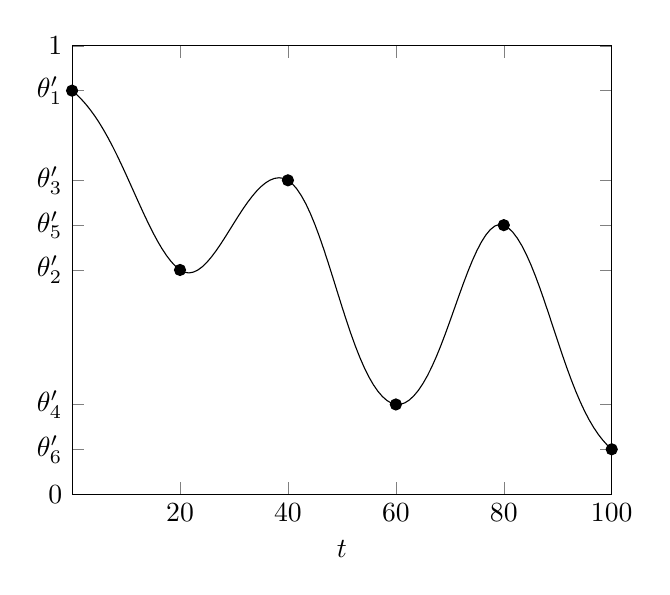
\begin{tikzpicture}
    \begin{axis}[xtick={20, 40,...,100}, ytick={0, 0.1, 0.2, 0.5, 0.6, 0.7, 0.9, 1}, yticklabels={0, $\theta_6'$, $\theta_4'$, $\theta_2'$, $\theta_5'$, $\theta_3'$, $\theta_1'$, 1}, xmin=0, xmax=100,  ymin=0, ymax=1, xlabel = $t$]

\addplot[domain=0:20] {1/(1+e^(-((2*((x-0)/(20-0))^3 - 3*((x-0)/(20-0))^2 + 1)*(2.2) + (((x-0)/(20-0))^3 - 2*((x-0)/(20-0))^2+((x-0)/(20-0)))*(0-(2.2)) + (-2*((x-0)/(20-0))^3+3*((x-0)/(20-0))^2)*(0) + (((x-0)/(20-0))^3-((x-0)/(20-0))^2)*1/2*((0-2.2) + (0.8473-0)) )))};
\addplot[domain=20:40] {1/(1+e^(-((2*((x-20)/(40-20))^3 - 3*((x-20)/(40-20))^2 + 1)*0 + (((x-20)/(40-20))^3 - 2*((x-20)/(40-20))^2+((x-20)/(40-20)))*1/2*( (0.8473-0) + (0-(2.2)))+ (-2*((x-20)/(40-20))^3+3*((x-20)/(40-20))^2)*(0.8473) + (((x-20)/(40-20))^3-((x-20)/(40-20))^2)*1/2*((0.8473-0) + (-(1.3863)-0.8473)) )))};
\addplot[domain=40:60] {1/(1+e^(-((2*((x-40)/(60-40))^3 - 3*((x-40)/(60-40))^2 + 1)*0.8473 + (((x-40)/(60-40))^3 - 2*((x-40)/(60-40))^2+((x-40)/(60-40)))*1/2*( (-(1.3863)-0.8473) + (0.8473-0))+ (-2*((x-40)/(60-40))^3+3*((x-40)/(60-40))^2)*(-(1.3863)) + (((x-40)/(60-40))^3-((x-40)/(60-40))^2)*1/2*((-(1.3863)-0.8473) + (0.4054--(1.3863))) )))};
\addplot[domain=60:80] {1/(1+e^(-((2*((x-60)/(80-60))^3 - 3*((x-60)/(80-60))^2 + 1)*-(1.3863) + (((x-60)/(80-60))^3 - 2*((x-60)/(80-60))^2+((x-60)/(80-60)))*1/2*( (0.4054--(1.3863)) + (-(1.3863)-0.8473))+ (-2*((x-60)/(80-60))^3+3*((x-60)/(80-60))^2)*(0.4054) + (((x-60)/(80-60))^3-((x-60)/(80-60))^2)*1/2*((0.4054--(1.3863)) + (-2.1972-0.4054)) )))};
\addplot[domain=80:100] {1/(1+e^(-((2*((x-80)/(100-80))^3 - 3*((x-80)/(100-80))^2 + 1)*0.4054 + (((x-80)/(100-80))^3 - 2*((x-80)/(100-80))^2+((x-80)/(100-80)))*1/2*( (-2.1972-0.4054) + (0.4054--(1.3863)))+ (-2*((x-80)/(100-80))^3+3*((x-80)/(100-80))^2)*(-2.1972) + (((x-80)/(100-80))^3-((x-80)/(100-80))^2)*1/2*((-2.1972-0.4054) + (0.2-2.1972)) )))};
\addplot[mark=*] coordinates {(0,0.9)};
\addplot[mark=*] coordinates {(20,0.5)};
\addplot[mark=*] coordinates {(40,0.7)};
\addplot[mark=*] coordinates {(60,0.2)};
\addplot[mark=*] coordinates {(100,0.1)};
\addplot[mark=*] coordinates {(80,0.6)};
\end{axis}
\end{tikzpicture}
}
\end{figure}



$f_{l}$ follows a spline $S(t)$ of order three that is transformed via the logistic function $\sigma(x)$ to obtain values between zero and one.
\begin{align}
f_{l}(\theta; t) =  \frac{1}{1 + \exp{(-P_{l,i}(t))}} \quad \forall t \in T_i. 
\end{align}
$P_{l,i}(t) \in \R_3(t)$ is a polynomial from the third order polynomial ring over the real numbers. We chose $P_{l,i}(t)$ to be in cubic hermite form, such that we can parameterize it by specifying the polynomial values at the boundaries 
\begin{align}
\label{eq:splines_bound_theta}
P_{l,i}(t_{i-1}) =& \theta_{l, i-1} \\
P_{l,i}(t_{i})=& \theta_{l,i} \notag
\end{align}
and using finite differences as approximations of the derivatives $P_{l,i}'(t)$. To compute the approximations, we use central finite differences and forward as well as backward finite differences at the respective boundaries $t_0$ and $t_{z}$
\begin{align}
\label{eq:finite_differences}
P'_{l,1}(t_0) &\approx \frac{P_{l,1}(t_1) - P_{l,1}(t_0)}{t_1 - t_0} \\
P'_{l,i}(t_{i-1}) &\approx \frac{1}{2}\left[\frac{P_{l,i}(t_{i}) - P_{l,i}(t_{i-1})}{t_{i} - t_{i-1}} + \frac{P_{l,i-1}(t_{i-1}) - P_{l,i-1}( t_{i-2})}{t_{i-1} - t_{i-2}} \right] \notag \\
P'_{l,z}(t_{z}) &\approx \frac{P_{l,z}(t_{z}) - P_{l,z}(t_{z-1})}{t_{z} - t_{z-1}} \notag 
\end{align}
Let $t' = (t-t_{i-1})/(t_{i} - t_{i-1})$. The polynomial $P_{l,i}(t) $ is given as a linear combination of four basis polynomials  $B_1(t), B_2(t), B_3(t), B_4(t) \in \R_3(t)$ with the boundary values of the polynomial and its derivative
\begin{align}
P_{l,i}(t) &= B_1(t') \overbrace{P_{l,i}(t_{i-1})}^{\theta_{l,i-1}} + B_2(t') (t_{i} - t_{i-1}) P'_{l,i}(t_{i-1})  \\& \quad + B_3(t') \underbrace{P_{l,i}(t_{i})}_{\theta_{l,i}} + B_4(t') (t_{i} - t_{i-1}) P'_{l,i}(t_{i}) \quad \forall t \in T_i. \notag
\end{align}
The scalars are dependent on the parameter vector $\theta_l$ through \eqref{eq:splines_bound_theta} and \eqref{eq:finite_differences}. The basis polynomials are defined by$B_1(t) = 2t^3 - 3t^2 +1, B_2(t) = t^3 - 2t^2 +t, B_3(t) = -2t^3 + 3t^2$ and $B_4(t) = t^3 - t^2$. We show subsequently that they indeed form a basis of $\R_3(t)$. Showing the basis property aims to proof that the four polynomials span $\R_3(t)$ and we therefore do not exclude any polynomials from the space of policies that could be implemented.
\begin{theorem}
$B_1(t), B_2(t), B_3(t), B_4(t) \in \R_3(t)$ form a polynomial basis of $\R_3(t)$.
\end{theorem}
\begin{proof}
We need to show that the four polynomials are linearly independent. We do so by writing the polynomials in vector form, collect them in a matrix and show that this matrix has full rank. 
\begin{align*}
\begin{pmatrix}
2 & 1 & -2 & 1\\
-3 & -2 & 3 & -1 \\
0 & 1 & 0 & 0 \\
1 & 0 & 0 & 0 \\
\end{pmatrix}
\Leftrightarrow
\begin{pmatrix}
0 & 0 & -2 & 1\\
0 & 0 & 1 & -1 \\
0 & 1 & 0 & 0 \\
1 & 0 & 0 & 0 \\
\end{pmatrix}
\Leftrightarrow
\begin{pmatrix}
0 & 0 & 0 & -1\\
0 & 0 & 1 & -1 \\
0 & 1 & 0 & 0 \\
1 & 0 & 0 & 0 \\
\end{pmatrix}
\Leftrightarrow
\begin{pmatrix}
0 & 0 & 0 & 1\\
0 & 0 & 1 & 0 \\
0 & 1 & 0 & 0 \\
1 & 0 & 0 & 0 \\
\end{pmatrix}
\end{align*}
Since $B_1(t), B_2(t), B_3(t), B_4(t)$ are four linearly independent polynomials of degree 3, they form a basis of $\R_3(t)$. 
\end{proof} 

\textbf{Neural network.} 

 
